% This is a sample document using the University of Minnesota, Morris, Computer Science
% Senior Seminar modification of the ACM sig-alternate style. Much of this content is taken
% directly from the ACM sample document illustrating the use of the sig-alternate class. Certain
% parts that we never use have been removed to simplify the example, and a few additional
% components have been added.

% See https://github.com/UMM-CSci/Senior_seminar_templates for more info and to make
% suggestions and corrections.

\documentclass{sig-alternate}
\usepackage{color}
\usepackage[colorinlistoftodos]{todonotes}

\newcommand{\comment}[1]{}
\definecolor{Coquelicot}{RGB}{255, 56, 0}
\newcommand{\pscomment}[1]{\textcolor{Coquelicot}{\comment{Paul: {#1}}}}

%%%%% Uncomment the following line and comment out the previous one
%%%%% to remove all comments
%%%%% NOTE: comments still occupy a line even if invisible;
%%%%% Don't write them as a separate paragraph
%\newcommand{\mycomment}[1]{}

\begin{document}

% --- Author Metadata here ---
%%% REMEMBER TO CHANGE THE SEMESTER AND YEAR
\conferenceinfo{UMM CSci Senior Seminar Conference, December 2013}{Morris, MN}

\title{Usability of Error Messages for Introductory Students}

\numberofauthors{1}

\author{
% The command \alignauthor (no curly braces needed) should
% precede each author name, affiliation/snail-mail address and
% e-mail address. Additionally, tag each line of
% affiliation/address with \affaddr, and tag the
% e-mail address with \email.
\alignauthor
Paul A. Schliep\\
	\affaddr{Division of Science and Mathematics}\\
	\affaddr{University of Minnesota, Morris}\\
	\affaddr{Morris, Minnesota, USA 56267}\\
	\email{schli202@morris.umn.edu}
}

\maketitle
\begin{abstract}
Error messages are an important tool for programmers to help find and fix mistakes or issues in their code.
When an error message is unhelpful, it can be difficult to find the issue and may impose learning difficulties.
Error messages are especially critical for introductory programmers in understanding problems with their code.
Not all error messages are beneficial for helping novice programmers, however.
This paper discusses the general usability of error messages for introductory programmers, analyses of error messages in compilers and DrRacket, and two methodologies meant to improve error handling.

% The current paper format *only* allows inline comments using the todo
% macro. That's kind of a bummer, and it would be neat if someone figured
% out how to change the acmconf style to allow this. I suspect it isn't *hard*
% but there are quite a few details that have to be sorted out in synchrony.
\end{abstract}

\keywords{Novice programmers, usability, error messages, usability studies, compiler errors, syntax errors}


\section{Introduction}\label{sec:intro}
One of the most important foundations of computer programming is the communication between the system and the user, specifically in the error messages produced by the system.
These error messages are especially important for introductory-level computer science students to help them resolve issues in their program because the error messages are the primary source for understanding what is wrong.
According to Marceau et al., ``[students] lack the experience to decipher complicated or poorly-constructed feedback''~\cite{Marceau:2011:MEE:1953163.1953308}.
The first rule of good message design is to be sure that the error does not add confusion~\cite{Isa:1983:MOE:800045.801583}.
Difficulties in understanding error messages often lead to frustration because the error message was either too complicated to understand or led them down the wrong path~\cite{Marceau:2011:MYL:2048237.2048241}, which can sometimes introduce new errors~\cite{Denny:2014:ESE:2591708.2591748}.

Various studies have been conducted on modern programming languages' error messages to study the effectiveness in helping novice programmers debug their program and help learn the concepts and programming languages.
The results have shown that students struggle with various elements of error messages such as terminology source highlighting~\cite{Denny:2014:ESE:2591708.2591748,Traver:2010} (which we discuss in detail in Section \ref{sec:analyses}).
Several tools and heuristics are being developed to help address issues in error message usability.
The goals of these methodologies are to help introductory programmers learn the language and concepts easier and more easily guide the programmers to a solution.
The purpose of this paper is to discuss analyses of error message design and its usability for introductory students in a class setting (meaning students' interactions with programming in a lab setting and at home), and how these developed methodologies help improve the user experience with error messages. 

This paper is divided into four sections.
In Section \ref{sec:background} we discuss usability studies, and then define compiler, syntax, and runtime error messages. After that, we introduce static and dynamic languages, and discuss imperative and functional programming. We then define interactive development environments and proceed to introduce the tools covered in the analyses used in Section \ref{sec:analyses}.
In Section \ref{sec:analyses} we focus on analyses of the usability of error messages in development environments and compiler messages for introductory students and how those analyses were performed.
In Section \ref{sec:methodologies} we examine Marceau et al.'s recommendations for error message design~\cite{Marceau:2011:MYL:2048237.2048241} and then we explore Denny et al.'s syntax error enhancement tool~\cite{Denny:2014:ESE:2591708.2591748}.


\section{Background}\label{sec:background}
In order to discuss the analyses of error messages, we need to understand several concepts related to error types and usability.
These concepts include compiler errors, syntax errors, runtime errors, usability studies, and Human Computer Interaction.
We also define dynamically and statically typed languages and their differences.
We then discuss the programming languages and tools used in the analysis of the error messages.
We will focus on the Racket, C++, and Java programming languages and the integrated development environment (IDE) DrRacket.


\subsection{Human-computer interaction and methods of usability analysis}\label{subsec:hci}

The study of Human-Computer Interaction, or HCI, is focused on how computer technology is used, specifically on the interfaces between the user and the programs on the computer.
As Traver notes, ``HCI is a discipline that aims to provide user interfaces that make working with a computer a more productive, effective, and enjoyable task''~\cite{Traver:2010}.
Much of the research presented in this paper is viewed from an HCI perspective and emphasized usability.

In order to analyze these messages from an HCI perspective and attain qualitative and quantitative information about their usability, a case study may be performed.
A case study is a research method that closely studies a group of participants, in the case of this paper, introductory students in a classroom, and collects data about participants by observations and interviews. 
Many of the studies performed on error messages analyzed in this paper are using a case study design.
Through these case studies, a t-test may be done, which is a test to find significance between two sets of data.
The significance in a t-test is determined by the computed p-value, which is the value that shows the level of significance.
In this paper, a p-value > 0.05 will be considered significant.

\subsection{Compiler and Runtime errors}\label{subsec:error types}

%I put this here to get it to display on the right page, oh LaTeX!
\begin{figure*}\label{fig:drracketdata}
  \centering
  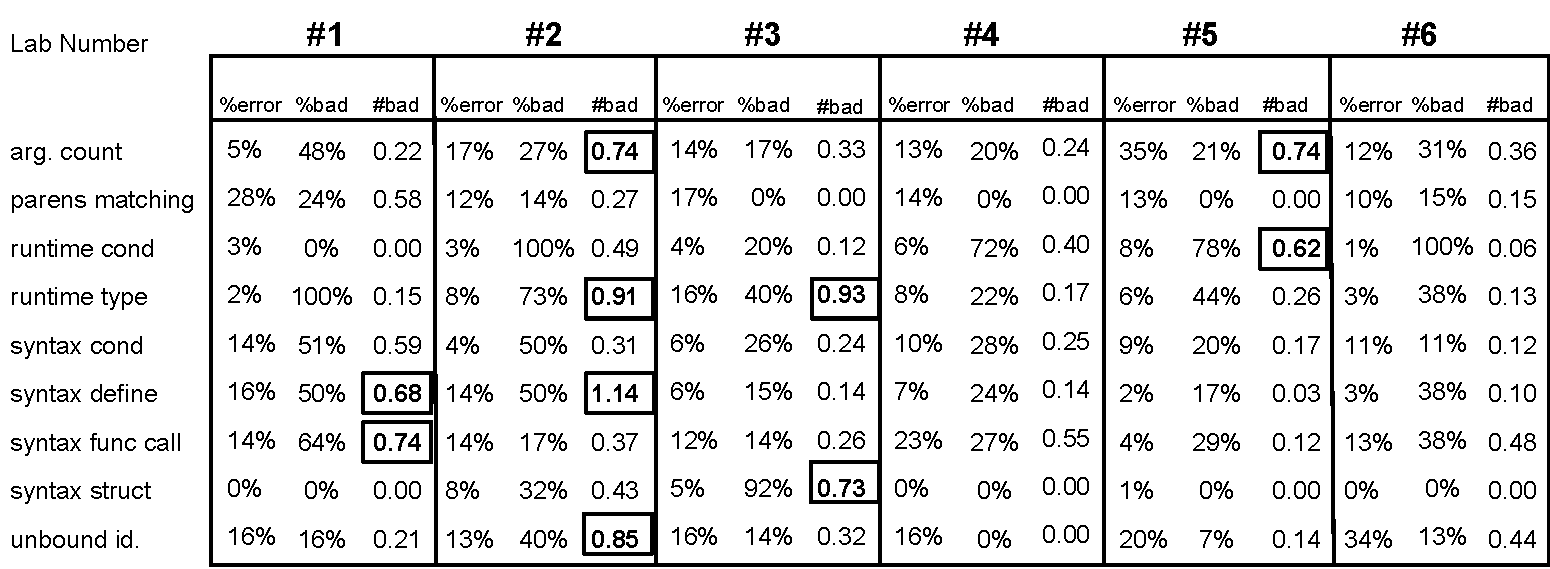
\includegraphics[keepaspectratio, width= 1.0 \textwidth]{MEE-Data.pdf}
  \caption{Results from DrRacket study}
  \label{fig:drracketstudy}
\end{figure*}

When writing code, a programmer may receive various error messages during different phases of the program, runtime and compile time.
A compiler is a program that converts source code written in a programming language into a language that a computer's processor can read so that instructions can be executed.
A compilation error refers to a state when a compiler fails to compile a piece of  program source code.
A program will not run if there is a compiler error because the compiler will not be able to create executable code to run if there are errors the compiler finds. 

Then, we examine syntax errors, which is a type of compiler error that occurs when the code does not conform to the syntactical order expected by the parser.
The parser, is a program (usually part of a compiler) that receives input as source code and builds it into a structural representation of the input while checking for correct syntax of the input.
As Kummerfield and Kay note, ``The usability of compiler errors are important because syntax error correction is the first step in the debugging process. It is not possible to continue program development until the code compiles. This means it is a crucial part of the error correction process.''~\cite{Kummerfeld:2003:NBF:858403.858416}

Below is an example of a compiler error in Java. Here, the programmer is defining \texttt{seven} to be \texttt{2+5}, but forgot to close the parenthesis. The compiler caught the syntax error, so the program did not execute.

\begin{verbatim}
int seven = (2 + 5;

error: ')' expected
\end{verbatim}

A runtime error is when there is an error detected when the program is executed.
Runtime errors often indicate problems in the logic of the program such as running out of memory and can be harder to find and debug, but can also occur from unforeseen circumstances such as hardware issues.
Below is an example of a runtime error in Java.
Here, the user wanted to print out a part of the string, "Hello World" but had the wrong bounds in the substring command (which returns a substring of a string).
The error is telling the programmer that the wrong bounds are given and are out of the range of the string "Hello World" where the programmer should have given the bounds of \texttt{(6,11)}.

\begin{verbatim}
String string = "Hello World";
System.out.print(string.substring(6,12));

java.lang.StringIndexOutOfBoundsException:
String index out of range: 12
\end{verbatim}

\subsection{Overview of programming languages and tools analyzed}\label{subsec:languages}

In section \ref{sec:analyses}, we discuss a study performed by Marceau et al. that analyzes the error messages in the DrRacket integrated development environment~\cite{Marceau:2011:MEE:1953163.1953308}.
An integrated development environment, or IDE, is an application that has packaged several other programs typically consisting of a text editor, compiler, and other programs used to debug code.
An IDE is important for introductory programming classes because they offer useful error reporting not seen in the language and can help a student debug their programs more easily.
For example, DrRacket offers highlighting offending line of code when the program fails and custom error messages geared specifically toward students.
DrRacket is an IDE meant for writing programs in Racket commonly geared toward introductory students and offers libraries for students to program at various levels.
These levels can produce more accessible error messages.

Racket is a member of the Lisp family of programming languages and is designed for programmers of various levels and is especially useful for introductory-level programmers.
Racket is a functional language, which means it uses a programming style of building elements of programs while retaining immutable data structures 
and without directly manipulating memory or changing state.
Functional languages generally work well in teaching programming concepts to students since functional approaches emphasize core computer science concepts such as recursion.
Racket is a dynamically typed language, which means a type is interpreted at runtime rather than compile time and variables in the language are not bound to types.
Thus it is possible in Racket to bind a name to variables of different types during the execution of a program since every variable name is bound only to an variables.
Since the runtime system of a dynamically typed language deduces type and type conversions, a programmer does not have to worry as much about type declaration.

We use C++ and Java in several examples throughout this paper.
C++ and Java are widely used programming languages not designed for introductory programming.
However, C++ and Java are often taught in a first computer science course.
C++ and Java are both imperative languages, which is a programming style that, as opposed to functional programming, uses a sequence of statements to build a computation using memory manipulation and changing the state of objects in a program.
These languages both fall in the style of Object-oriented programming, or OOP, which is a method of programming based on class hierarchy and is based around creating objects, which are data structures that contain a set of routines called methods. 
Java and C++ are statically typed languages, which means type checking is done at compile-time rather than runtime and objects are bound to types. 
This means that when programming in statically typed languages, a programmer may need to pay more attention to how types are cast, but provides benefits such as earlier detection of programming mistakes.

Since Java and C++ are statically typed languages, a programmer can receive type errors during compile time.
However, the same error will not occur in a dynamically typed language since type checking is done during runtime.
Consider the following example:

\begin{verbatim}
personName = "Francis"
personName = 7
\end{verbatim}

This sequence of statements is illegal in a statically typed language since we are binding a string to \texttt{personName}, then an integer to \texttt{personName}.
This statement would then throw an error during compile time.
This is a legal statement in a dynamically typed language, however, since variables don't have types in dynamic languages.
Note that this statement would not work in a purely function language since you can not change the value of a variable.


\section{Analyses}\label{sec:analyses}
In this section, we discuss two different studies performed on the usability of error messages and their results.
The first analysis will discuss how well the error messages in Racket and DrRacket help introductory students debug their programs.
The second analysis will discuss the effectiveness of compiler error messages in the C++ programming language. 


\subsection{Analysis of error messages in Racket and DrRacket}\label{subsec:racket analysis}

Marceau, Fisler, and Krishnamurthi helped design DrRacket's error messages so that they can be more helpful to beginner programmers.
However, Marceau et al. still noticed students struggling with debugging and understanding the error messages, so the authors were interested in seeing how their students responded to these error messages and to identify specific error messages that performed poorly~\cite{Marceau:2011:MYL:2048237.2048241}.
In the spring of 2010, Marceau, Fisler, and Krishnamurthi ran a case study on error messages in DrRacket.
The study involved configuring DrRacket to save a copy of each program a student tried to run as well as the error message through six 50 minute lab sessions~\cite{Marceau:2011:MEE:1953163.1953308}.
The authors were interested in which error messages are effective and how well DrRacket's text highlighting can help a student.  

In order to measure effectiveness, the authors developed a rubric which determined whether the student made a reasonable edit in response to the error message~\cite{Marceau:2011:MEE:1953163.1953308}.
The rubric was meant to distinguish how an error message would fail or succeed.
They determined that an error message is effective if a student can read it, understand it, and use that information to figure out how to resolve the issue.

The following Racket code, modified from~\cite{Marceau:2011:MEE:1953163.1953308}  shows an example of an error message in DrRacket that Marceau et al. found as not effective for helping a student debug their program.

\begin{verbatim}
(define (example name word1 word2)
   (cond
  	   (and (cond [(string=? name word1) "Name Located"]
                 [(string=? name word2) "Name Located"])
       "Mark")
))

-> and: found a use of `and' that does not follow 
an open parenthesis
\end{verbatim}

The message is contradicting the code as \texttt{and} does follow an open parenthesis, but the parser thinks \texttt{and} does not have an open parenthesis before it and claims that there needs to be an open parenthesis .
Unfortunately, to understand it, the programmer must realize that parser attributed the open parenthesis before the \texttt{and} to the \texttt{cond}.
The actual underlying issue is simply an extra closing parenthesis at the end of the definition, but trying to decipher that syntactical issue from the provided error message may be confusing to an introductory programmer.

%\begin{figure}[t!]
%  \centering
%  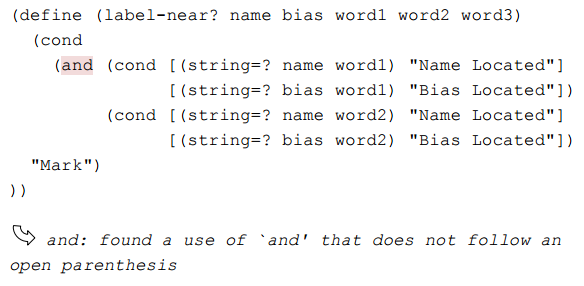
\includegraphics[keepaspectratio, width=0.5\textwidth]{MEE_example.png}
 % \caption{Example of an ineffective error message in Racket}
%  \label{fig:racketerrormessage}
%\end{figure}

%\todo[inline, color=orange]{simplify error message from figure 1, turn into verbatim}

Figure \ref{fig:drracketdata} shows the results (modified from~\cite{Marceau:2011:MEE:1953163.1953308}) of Marceau et al. study. 
They grouped messages into nine most common error categories in their results from the study, as seen on the left side of the table.
The top portion above the table shows the lab number.
Through their data collection at the end of the study, they found the percentage of occurrence of each error type from each lab as indicated by the \textit{\%error} and the percentage of students that responded poorly to the error message indicated as \textit{\%bad}, as seen in the top boxes of the table.
\textit{\#bad} shows the level of likelihood of recurrence of the respective error message.
The values of interest are the \textit{\#bad} values enclosed in a box and the highest \textit{\%bad} values, as seen in figure \ref{fig:drracketstudy}). 

The data the authors gathered helped identify errors students found challenging.
The authors found that students have difficulties with certain errors at different points in the course, as expected since curricular aspects of the labs affect error patterns.
Many of the errors students struggled with were consistent with the course, such as difficulties with syntax errors in the first lab since students are still beginning to learn the language syntax.

However, the data is not entirely a representation of students' conceptual difficulties with the course, as Marceau et al. found.
The error messages a student receives, according to Marceau et al., ``is often not a direct indicator of the underlying error''~\cite{Marceau:2011:MEE:1953163.1953308}.
For example, in lab number six, numerous \texttt{unbound-id} errors  or unbound identifiers occurred, which is when the compiler finds a variable that was not defined.
However, the authors found that the actual problem students had was improperly using field reference operators and the actual errors they should have received was not given.
This suggests that there are some issues in the effectiveness of the error messages.

\subsection{Analysis of compiler messages in C++}\label{subsec:compiler analysis}

Compiler error messages are often cryptic and difficult to understand for many programmers, especially for students who are new to programming.
Unfortunately, as Traver notes, ``most related disciplines, including compiler technology, have not paid much attention to this important aspect that affects programmers significantly, apparently because it is felt that programmers should adapt to compilers''~\cite{Traver:2010}.
Traver proposed to research compiler error message usability from a strictly HCI viewpoint.
So, we will not cover technical implications of developing error messages for compilers, but rather the how usable they are for helping introductory programmers resolve issues with their program.

In the first semester of 2002-2003, Traver conducted a case study on students' work with compiler error messages in C++ in an introductory computer science course.
The motivation of this study is to gain insight on what errors students are struggling with in the course.
Traver gathered data from the students' interactions with C++ throughout the semester and wrote up analyses of the error messages received in 5 separate parts.
\begin{itemize}
	\item \textit{The error message} received from the compiler
	\item \textit{The source code} that caused the original error
	\item \textit{The diagnostic} of why the error occurred
	\item \textit{An alternate error message} that may help lead more directly to the true diagnosis of the issue.
	\item \textit{A comment} about why the error message is not helpful
\end{itemize}

Below is an example of an error message in C++ analyzed in the study along with the source code that caused the error~\cite{Traver:2010} (in the interest of space,  have not included the other parts of the analysis):

Offending Code:
\begin{verbatim}
SavingAccount::SavingAccount(){
    float SavingAccount::getInterestRate() {
   	  return rate;
}
\end{verbatim}

Error Message:
\begin{verbatim}
In method 'SavingAccount::SavingAccount()':
declaration of 
'float SavingAccount::getInterestRate()'
outside of class is not definition
\end{verbatim}

In this case, the programmer forgot to close the curly bracket for the body of the method, so a syntax error would be thrown.
Although this is a relatively easy error to identify, when a program has multiple sets of braces, it can be easy to miss some braces along the way.
Traver found that this error message might not be suitable for every programmer because it does not provide any noticeable clues that the error is a missing bracket.
The author of the study noted that this type of error message should ``convey a clear message that the programmer can quickly understand and that is useful for fixing the error'', but the error message given to the user would not accomplish this for students who are still new to programming~\cite{Traver:2010}.

No quantitative data was gathered in this case study.
However, Traver found from this research (and previous research) that the usability of compiler errors is a well-known issue and they do not always properly tell the programmer the issue.
However, the author hopes that approaches (such as the syntax error message enhancement we cover in section \ref{sec:methodologies}) be considered to address the issues in compiler error message design.


\section{Methodologies}\label{sec:methodologies}
In this section, we discuss three methodologies and tools proposed to improve the usability of error messages or suggest improvements for error message design based on the analyses discussed in section \ref{sec:analyses}.
The first methodology we discuss is a set of recommendations for improving the usability of error messages in IDEs, specifically in DrRacket.
For the third approach, we will discuss an attempt on enhancing syntax error messages in Java and how well these syntax error messages improve over the original. 

\subsection{Recommendations for error messages in IDEs}\label{subsec:error message rubric}
After Marceau et al. analyzed their data from the case study (as detailed in section \ref{subsec:racket analysis}), they found that students struggled to respond to error messages.
Through their research, they were able to develop a list of proposed methods of improving error messages, specifically for DrRacket, ``but they should apply just as well in any other programming language used for teaching, including those with graphical syntaxes''~\cite{Marceau:2011:MYL:2048237.2048241}.
They also wanted to maintain two integral principles in error message design for their proposals:

\begin{itemize}
	\item Error messages should not propose solutions as these solutions can lead students down the wrong path and can not cover every scenario a student may encounter.
	\item Error messages should not prompt students toward incorrect edits. Source highlighting can cause issues and when not correctly implemented can cause more errors.
\end{itemize}

The first recommendation is simplifying vocabulary used in error messages.
The authors found that while DrRacket is ``accurate and consistent in its use of technical vocabulary'', but ``some of its terms are overly precise relative to terms that students already know''~\cite{Marceau:2011:MYL:2048237.2048241}.
For example, the term \texttt{identifier} is used in DrRacket error messages. However, the term \texttt{variable} is a term students are more likely to be familiar with~\cite{Marceau:2011:MYL:2048237.2048241}.
However, they also argue that non-simplified vocabulary is appropriate for an introductory computer science course, and thus decided this may be better suited in beginner levels of DrRacket.

Marceau et al. also wanted error messages to be explicit about inconsistencies, specifically with function or constructor usage.
They found that DrRacket highlights the source expression where the variable or constructor is called, but not the definition.
The highlighting suggest edits should be made in the expression, but the error can also occur within the definition of the variable or constructor, which does not get highlighted when an error like this occurs.
While an IDE may not be able to identify whether a definition or its usage is the issue, it should not steer students in the wrong direction~\cite{Marceau:2011:MYL:2048237.2048241}.

The authors then propose that error messages should highlight every reference and its corresponding code with a distinct color in order to help students match message terms to code fragments.
They believe this should help resolve ambiguity about highlighting and ambiguous references (an example of an ambiguous reference is highlighted in blue in figure \ref{fig:colorcodedmessage}).
Figure \ref{fig:colorcodedmessage} shows an example of a color coded error message, modified from~\cite{Marceau:2011:MYL:2048237.2048241}.
The red highlights the definition, the green highlights the clause, and the blue highlights the reference.

\begin{figure}
  \centering
  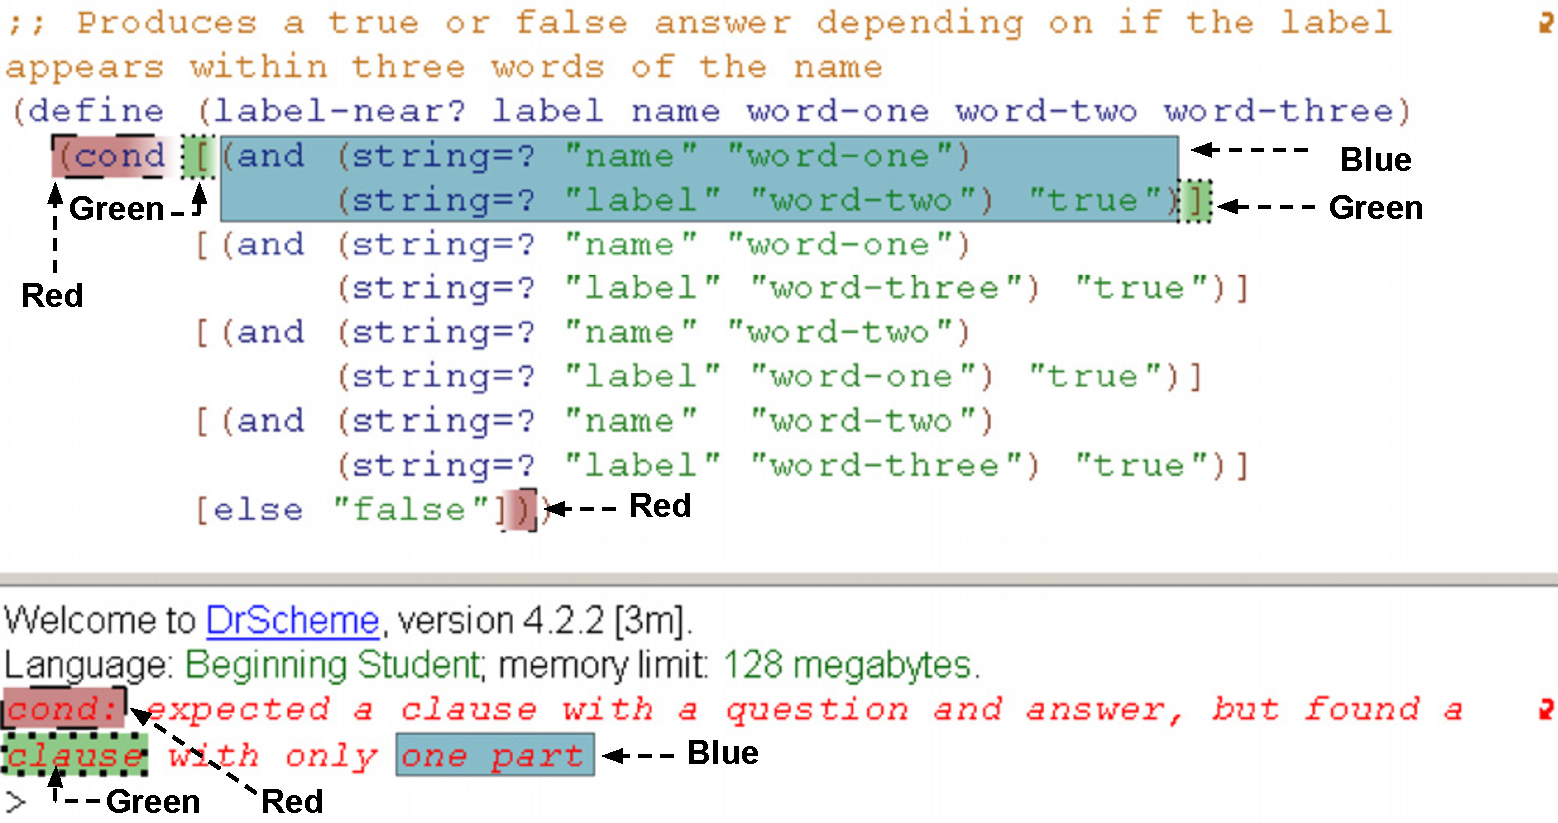
\includegraphics[keepaspectratio, width=0.50\textwidth]{ColorCodedMessage.pdf}
  \caption{Example of color coded message}
  \label{fig:colorcodedmessage}
\end{figure}

The last three recommendations are design suggestions for introductory courses that uses DrRacket to help students with error messages, so in the interest of space, we will not be covering them.
As of the writing of the paper, the authors had not implemented these suggestions, but do currently exist, which we discuss in section \ref{sec:ftrwrk}~\cite{Marceau:2011:MYL:2048237.2048241}. 


%\subsection{Principles of compiler error design}\label{subsec:compiler error design}
%\todo[inline, color=red]{TODO}

\subsection{Syntax error message enhancement and results}\label{subsec:syntax enhancement}

Language syntax is often one of the first difficulties a student experiences when learning programming~\cite{Denny:2011:USB:1999747.1999807}.
Because of this, introductory students may see many syntax errors while learning the syntax of a language.
Denny et al. found that ``syntax errors can be a significant barrier to student success'' and thus propose to improve the existing error messages that deal with syntactical issues in a Java-based development environment for introductory programmers~\cite{Denny:2014:ESE:2591708.2591748}.

Denny et al. decided to implement the enhanced error message system through CodeWrite, a web-based tool for students to complete various Java exercises.
The code is entered directly in the browser
The students need to write only the body of a method, the header of the method is always provided.
In order to create the enhanced feedback, the authors began by examining student submissions in CodeWrite and found the errors that had ambiguous compiler error messages. 
They achieved this by performing an analysis of the code and use regular expressions to match commonly occurring patterns of code that caused errors and  extracting the line containing the error.
They then categorized the error messages according to error type by building a program called a recognizer that would parse source code and raw compiler error messages.
Once the original error is extracted, they then highlight the line and insert their enhanced error message.
The enhanced error messages contain the line number of the offending line of code and a detailed explanation of the error.
They also show an example of incorrect code and correct code of the corresponding syntax error with an explanation.
Figure \ref{fig:ese} shows an example of an enhanced error message, modified from~\cite{Denny:2014:ESE:2591708.2591748} for readability.
This message was produced from the following erroneous code fragment:

\begin{verbatim}
if (score < 0) || (score > 100)
Syntax error on token "||", if expected
\end{verbatim}

This statement is syntactically incorrect because the \texttt{if} statement is missing surrounding parenthesis. The corrected statement is in the "Correct Code" block in figure \ref{fig:ese}.

\begin{figure*}
  \centering
  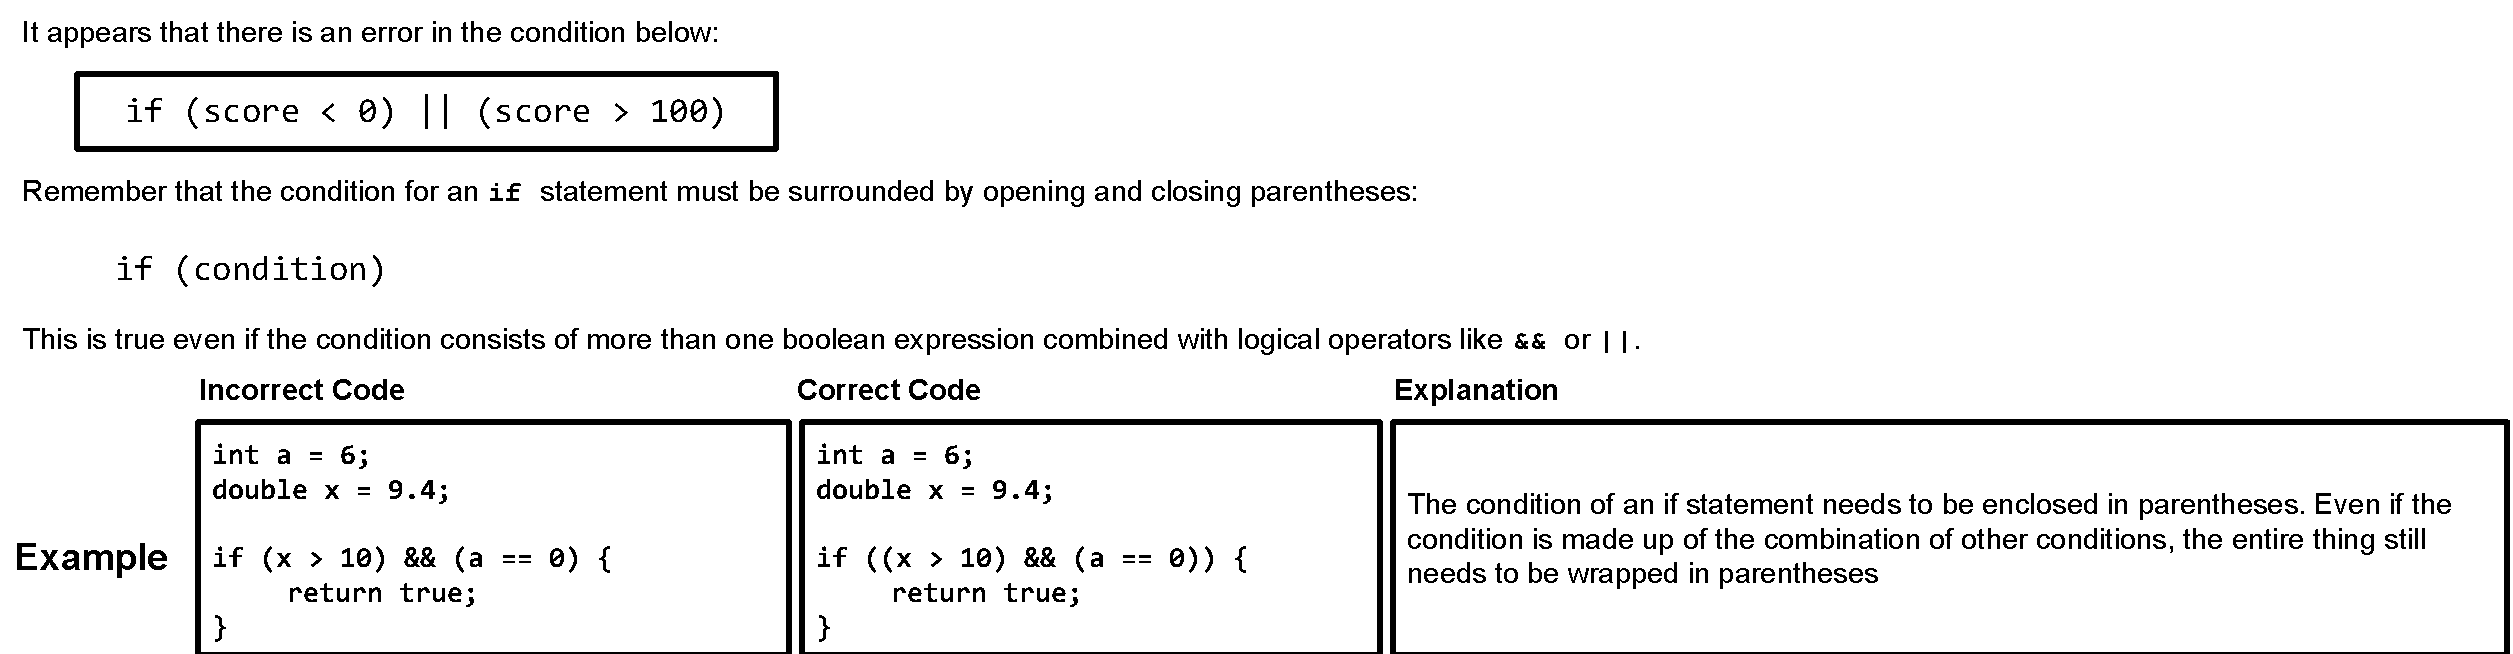
\includegraphics[keepaspectratio, width=\textwidth]{EnhancedSyntaxError.pdf}
  \caption{Example of an enhanced syntax error}
  \label{fig:ese}
\end{figure*}

The authors were interested in helping students improve their debugging skills, and were particularly interested in those who consistently submitted non-compiling code~\cite{Denny:2014:ESE:2591708.2591748}.
After creating these enhanced error messages, the authors wanted to examine whether they had an impact on:
\begin{itemize}
	\item The number of non-compiling submissions made while attempting an exercise
	\item The total number of non-compiling submissions
	\item The number of attempts needed to resolve most common kinds of errors
\end{itemize}

Denny et al. had students in a summer course randomly put in a control group that received the original error message or the intervention that received their new error messages and submit their code in CodeWrite where the authors could be able to compare the submissions of the same exercise of each group.
Unfortunately, after testing whether their enhanced error messages had an impact on the above items, they found that their new feedback had no significant differences between the groups.

Denny et al. measured the effectiveness by comparing the attempts of students submissions, specifically looking for syntax errors.
Denny et al. ran a t-test to see if their program would reduce the nubmer of non-compiling submissions while attempting an exercise.
They found for each problem a p-value > 0.05, which means there was no significant differences between the groups.
Denny et al. found similar results for whether their program would reduce the total number of non-compiling submissions.
The t-test gave a p-value = 0.9471, showing non-significance.
Finally, they tested whether their program reduced the number of attempts needed to resolve the most common kind of errors (variable undefined, type error, missing semicolon).
Again, they found for each case, the p-value was large and thus their program had no significant effect.

Denny et al. found numerous possibilities for why their enhanced feedback system was not effective on helping introductory students improve their debugging skills.
They believed that the errors could have been simple enough to solve without needing to look at the messages.
Another possibility was that students did not put more attention into the additional information of the messages.
The authors hope to apply additional research into their enhanced errors to further find out why they were not any more helpful than the original messages~\cite{Denny:2014:ESE:2591708.2591748}.


\section{Conclusion}\label{sec:concl}

In this paper, we discussed studies done on error messages in DrRacket and compiler error messages and how well introductory students can use them for debugging.
The research on DrRacket error messages found that students have difficulties with understanding error messages on unfamiliar concepts.
However, some errors in DrRacket incorrectly report the problem to the students and thus there is room for improvement.
The analysis on compiler error messages deduced that compiler messages are generally unusable for introductory programmers.

However, there is research being done on attempting to improve or suggest the improvement for the usability of error messages.
We discussed a set of recommendations on designing error messages toward introductory students.
We also discussed a system of enhanced error messages for syntactical issues, but was found ineffective at being more helpful than the original messages.

\section{Future work}\label{sec:ftrwrk}

Marceau et al. created a series of recommendations that they have implemented in HtDP libraries for DrRacket.
HtDP, or How to Design Programs, is a library that offers the enhancements of error messages detailed in subsection \ref{subsec:error message rubric} and constructs the language features to help restrict the set of explanations for student errors.
This library requires further research to find the effectiveness this has for introductory students~\cite{htdp-teachpacks}.

Traver noted in his research on compiler errors that some approaches have been made to attempt to make these messages better communicate the problem to the programmer, such as Denny et al.'s syntax error enhancement, but ``the problem is far from being properly solved''~\cite{Traver:2010}. 
Traver hopes ``that state-of-the-art compilers will advance towards smart, very programmer-friendly compilers.''
While it is crucial to retain an error message's educational standpoint, it is also important to ease new students into learning a programming language.
So, making sure the messages are user-friendly, such as familiar vocabulary or showing hints, is imperative to giving useful feedback for introductory students so they can more easily understand the programming language.


% The following two commands are all you need in the
% initial runs of your .tex file to
% produce the bibliography for the citations in your paper.
\bibliographystyle{acm}
% sample_paper.bib is the name of the BibTex file containing the
% bibliography entries. Note that you *don't* include the .bib ending here.
\bibliography{Usability_of_Error_Messages_for_Novice_Programmers}  

%\todo[inline, color=blue]{Citing sources for references}
%~\cite{Denny:2014:ESE:2591708.2591748}
%~\cite{Hartmann:2010:OPS:1753326.1753478}
%~\cite{Isa:1983:MOE:800045.801583}
%~\cite{Kummerfeld:2003:NBF:858403.858416}
%~\cite{Marceau:2011:MEE:1953163.1953308}
%~\cite{Marceau:2011:MYL:2048237.2048241}
%~\cite{Murphy:2008:BTD:1352135.1352193}
%~\cite{Traver:2010}
%~\cite{Denny:2011:USB:1999747.1999807}
% You must have a proper ".bib" file
%  and remember to run:
% latex bibtex latex latex
% to resolve all references

\end{document}
